\chapter{Introducción}
\label{cap:introduccion}
\setcounter{page}{1}

El avance tecnológico constante ha transformado nuestra forma de percibir el mundo. El continuo desarrollo en campos como la robótica, ha dado lugar a dispositivos capaces de realizar tareas que antes parecían imposibles. Hace medio siglo, la idea de un dispositivo que fuera capaz de barrer de forma eficiente o de un vehículo que se condujera solo era imposible de imaginar. Hoy en día, los vehículos inteligentes han pasado de formar parte de ciencia ficción a convertirse en una realidad que está revolucionando el transporte y remodelando nuestras ciudades. Por ejemplo, en algunas ciudades de Estados Unidos ya hay robo-taxis sin conductor que circulan de forma completamente autónoma transportando pasajeros.

La capacidad de los vehículos autónomos para desenvolverse de manera segura en entornos complejos, no solo reduce los errores humanos\footnote{\url{https://www.tesla.com/es_es/VehicleSafetyReport}}, sino que también abre nuevas oportunidades en ámbitos esenciales. Desde mejorar la seguridad vial y promover la eficiencia energética hasta fomentar la inclusión social, convirtiéndose en pilares fundamentales para el desarrollo de ciudades más sostenibles. Estos vehículos podrían contribuir significativamente a la reducción de emisiones contaminantes, impactando positivamente en la calidad del aire urbano; al mismo tiempo que las personas con movilidad reducida o dificultades para conducir podrían tener un acceso más equitativo a los servicios de transporte. Conseguiríamos una movilidad inclusiva, eliminando incluso la necesidad de contar con un carnet de conducir para desplazarse en coche. Aunque todavía queda un largo camino por recorrer, los avances actuales permiten vislumbrar un futuro donde el tráfico sea más fluido y los recursos urbanos se utilicen de forma más eficiente. Además, gracias a su capacidad de comunicarse entre sí mediante la tecnología \ac{V2V}\footnote{\url{https://arxiv.org/pdf/2102.07306}}, estos vehículos podrían coordinar aspectos como la velocidad y la dirección, optimizando los tiempos de viaje y disminuyendo la congestión de tráfico en grandes ciudades.

\section{Vehículos autónomos}
\label{sec:vehículos}

Un vehículo autónomo es aquel capaz de realizar todas las funciones de conducción sin necesidad de intervención humana, más allá de indicar el inicio y el final del trayecto. Estos vehículos se caracterizan por operar de manera más eficiente, segura y sostenible que los automóviles convencionales, gracias al uso de tecnologías avanzadas como sensores, cámaras, radares y algoritmos de \ac{IA}. Sin embargo, en los niveles intermedios de autonomía, aún se requiere la participación del conductor en ciertas situaciones, ya que el vehículo actúa como un asistente que puede tomar el control en casos específicos, pero sigue dependiendo de la supervisión humana.

En la actualidad, la industria automotriz ha desarrollado una amplia gama de \ac{ADAS}, cuyo objetivo principal es reducir el riesgo de accidentes mediante la ayuda a los conductores. Estos sistemas emplean una red de sensores para analizar el entorno de conducción, procesando la información a través de la electrónica del vehículo, lo que les permite tomar decisiones predefinidas e intervenir en elementos como el acelerador, los frenos o la dirección. \textit{Toyota}, por ejemplo, incluye en sus vehículos una gran variedad de \ac{ADAS}: el control de crucero adaptativo, reconocimiento de señales de tráfico, control de trayectoria, control inteligente de luces en la carretera, un sistema avanzado de aparcamiento inteligente y sistema de seguridad precolisión, que alerta al conductor y asiste en el frenado monitoreando tanto en la parte trasera como delantera del coche \cite{toyota-assist}. Otras marcas como \textit{Audi}, con su modelo A4\footnote{\url{https://www.audi.es/es/modelos/a4/a4/}} y \textit{BMW}\footnote{\url{https://www.bmwautomotor.com/que-significan-los-sistemas-adas-para-el-coche/}}, también destacan con sistemas sofisticados. Aunque estos logros representan pasos intermedios hacia la conducción autónoma completa, los \ac{ADAS} continúan asistiendo al conductor en tareas específicas, aún requieren su supervisión activa. Los \ac{ADAS} establecen las bases para la implementación futura de sistemas totalmente autónomos. 

En este contexto de avances continuos en la conducción autónoma, la Sociedad de Ingenieros Automotrices (\ac{SAE}) ha establecido una clasificación estandarizada de los niveles de autonomía de los vehículos, que abarca desde la conducción completamente manual hasta la conducción completamente autónoma. Esta categorización divide los vehículos autónomos en seis niveles según el grado de intervención requerido por el conductor y la capacidad del sistema del vehículo para tomar control \cite{autobild-autonomous}.

\newpage

\begin{figure} [ht]
\begin{center}
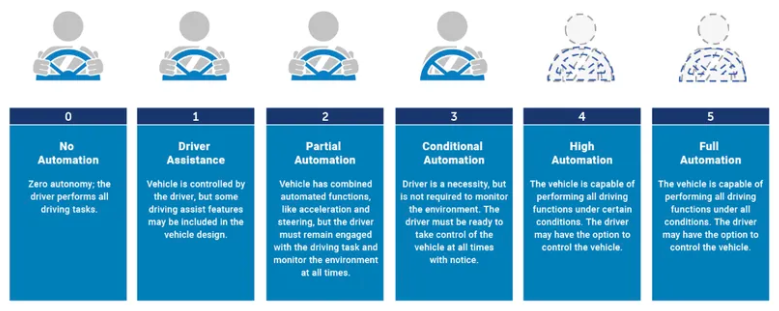
\includegraphics[width=13cm]{figs/introducción/niveles.png}
\end{center}
\caption{Niveles de autonomía explicados(\ac{SAE}) \cite{autobild-autonomous}.}
\label{aut-levels}
\end{figure}

\begin{itemize}
\item \textit{Nivel 0:} Ninguna autonomía. El conductor es completamente responsable de todas las tareas de conducción.
\item \textit{Nivel 1:} Asistencia al conductor. El vehículo puede realizar una función específica (como el control de crucero), pero siempre requiere la supervisión activa del conductor.
\item \textit{Nivel 2:} Automatización parcial. El vehículo cuenta con sistemas que pueden realizar tareas de conducción, pero el conductor debe estar preparado para intervenir en cualquier momento.
\item \textit{Nivel 3:} Automatización condicional. El vehículo puede tomar el control completo en determinadas condiciones, pero el conductor debe estar disponible para retomarlo si el sistema lo solicita.
\item \textit{Nivel 4:} Alta automatización. El vehículo puede operar de forma autónoma en condiciones específicas, sin necesidad de intervención humana, aunque pueden existir limitaciones geográficas o contextuales.
\item \textit{Nivel 5:} Automatización total. El vehículo es completamente autónomo y no requiere la intervención humana en ningún momento ni bajo ninguna circunstancia.
\end{itemize}

Hoy en día, no existen vehículos completamente autónomos (nivel 5) circulando por las carreteras o disponibles comercialmente. Normalmente en el mercado encontramos coches autónomos de nivel 2+ e incluso 3. Puesto que, en muchos países, la legislación aún no permite el uso de vehículos autónomos de nivel 3 o superior. Por ejemplo, en España, la ley prohíbe que el conductor suelte el volante durante la conducción, lo que impide el uso de vehículos de nivel 3. En cambio, en regiones de Estados Unidos, es legal el uso de vehículos con conducción semi-autónoma, lo que permite al conductor levantar las manos del volante en ciertas circunstancias e incluso vehículos sin conductor \cite{carwow-autonomous}. Existen numerosos proyectos que ofrecen un nivel 4 de autonomía y ya se están probando en entornos urbanos reales, como los robo-taxis de \textit{Waymo} en California. 

A pesar de la legislación española actual, se están realizando nuevas propuestas y proyectos para fomentar el uso y desarrollo de vehículos con mayor nivel de autonomía. El gobierno de la Comunidad de Madrid ha presentado un borrador para una nueva Ley de Movilidad que fomente el despliegue de vehículos autónomos por la ciudad, con el objetivo de mejorar la movilidad, reducir los atascos e impulsar un Madrid más sostenible \cite{com-madrid}. La localidad de Leganés es pionera en el despliegue de vehículos sin conductor, a finales de enero de 2025 un autobús urbano sin conductor recorrió 2,3 kilómetros realizando cuatro paradas para recoger nuevos pasajeros en el barrio de Leganés Norte. Estos autobuses ya funcionan en países como Noruega y Finlandia, comprobando que reducen los tiempos de espera y la probabilidad de accidentes. Leganés prevé seguir fomentando este tipo de iniciativas y modernizando su transporte urbano con la colaboración de la universidad Carlos III de Madrid, ubica en dicha localidad \cite{leganes}.
\begin{figure} [ht]
\begin{center}
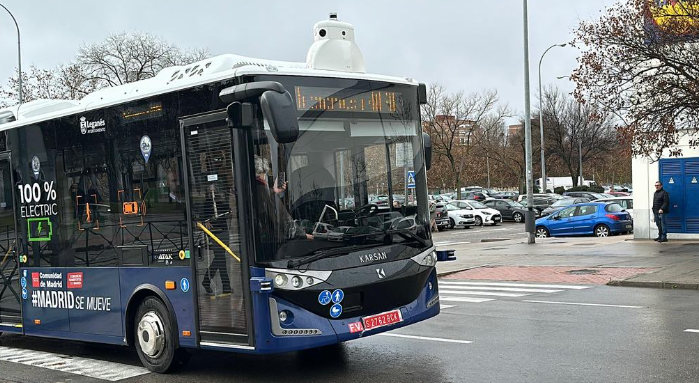
\includegraphics[width=8cm]{figs/introducción/bus_leganes.png}
\end{center}
\caption{Autobús sin conductor en la localidad de Leganés.}
\label{leganes-photo}
\end{figure}

\subsection{Evolución histórica de los vehículos autónomos}
\label{sec:historia}

La primera vez que se puso en práctica el concepto de vehículo autónomo fue en 1925 en Nueva York. El ingeniero Francis Houdina diseñó el primer coche sin conductor, controlado de forma remota por radiofrecuencia. Sin embargo, este vehículo requería otro vehículo escolta desde el cual se dirigía.

En 1939, el diseñador industrial estadounidense Norman Bel Geddes revolucionó las ideas sobre transporte al presentar en la Feria Futurama un concepto visionario: vehículos eléctricos guiados de manera autónoma mediante radiocontrol en carreteras automáticas con circuitos eléctricos integrados en el pavimento. Aunque no se trataba del concepto moderno de coche autónomo, esta propuesta marcó un antes y un después, despertando el interés de numerosas empresas tecnológicas en el campo de la conducción autónoma.

\begin{figure} [ht]
\begin{center}
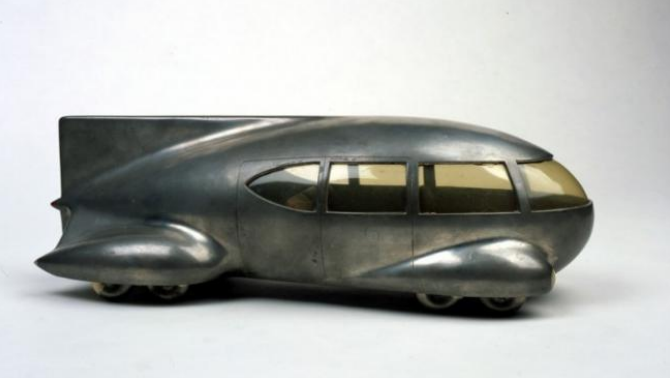
\includegraphics[width=8cm]{figs/introducción/coche_geddes.png}
\end{center}
\caption{Coche diseñado por Norman Bel Geddes en 1933 \cite{bel-geddes}.}
\label{coche-geddes}
\end{figure}

La mayoría de los avances significativos en este ámbito se deben a Ernst Dickmanns, un profesor alemán experto en \ac{IA}. Dickmanns lideró la creación del primer coche autónomo moderno, combinando la visión sacádica (un movimiento
rápido del ojo, cabeza u otras partes del cuerpo de animales o dispositivos) con cálculos probabilísticos y computación paralela. En 1987, diseñó una furgoneta \textit{Mercedes-Benz} equipada con esta tecnología, logrando conducirla con éxito por una autopista a velocidades de hasta 100 km/h en condiciones de tráfico controladas. En 1994, lo superó con el modelo \textit{Mercedes 500 SEL}, conocido como \textit{VaMP}, que recorrió más de 1.000 kilómetros en la carretera de circunvalación de París. Este vehículo alcanzó velocidades de hasta 130 km/h y era capaz de realizar maniobras complejas, como adelantamientos.

\begin{figure}[ht]
\begin{center}
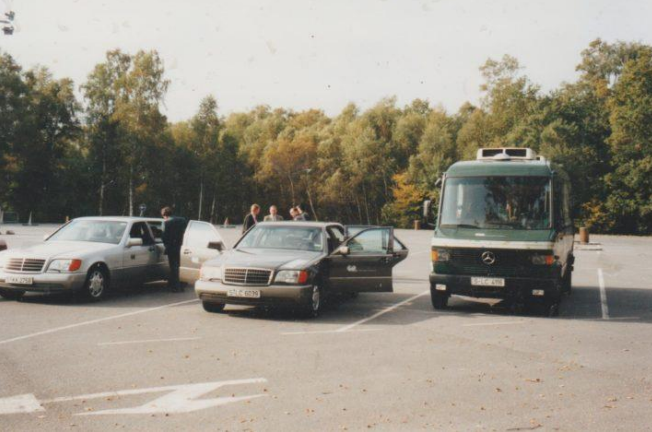
\includegraphics[width=7cm]{figs/introducción/paris_1994.png}
\end{center}
\caption{Demostración en vivo del funcionamiento de \textit{VaMP} en París \cite{dickmanns}.}
\label{coche-geddes}
\end{figure}

La Comisión Europea, consciente del potencial de los coches autónomos, destinó 800 millones de euros al proyecto \textit{EUREKA Prometheus}, una iniciativa que marcó un hito en el desarrollo de este tipo de tecnologías. Este programa facilitó la creación de numerosos prototipos que asentaron las bases de los vehículos autónomos modernos \cite{history-vehicles}. Actualmente, este campo es liderado por empresas como \textit{Waymo}, \textit{Tesla}, \textit{Cruise} y \textit{Baiud}.

\subsubsection{Waymo}

\textit{Waymo} \footnote{\url{https://waymo.com/intl/es/}}, el sistema de conducción autónoma desarrollado por \textit{ Google}, se ha consolidado como un referente en el sector de los vehículos sin conductor. El proyecto, que comenzó en 2009 bajo el nombre de \textit{Google Self-Driving Car Project}, fue rebautizado en 2016 como {Waymo}. Desde entonces, ha avanzado notablemente, destacando por su capacidad para integrar la \ac{IA} en sus vehículos, lo que les permite planificar rutas complejas y reaccionar de manera inteligente ante diversos escenarios en la carretera. Los vehículos de \textit{Waymo} operan en un Nivel 4 de autonomía \footnote{\url {https://skiller.education/waymo}}, son capaces de manejar la mayoría de las situaciones de conducción sin intervención humana. Sin embargo, aún existen localizaciones y escenarios complejos en los que aún no se consigue un comportamiento adecuado y eficiente.

Un vehículo \textit{Waymo} es capaz de operar de manera segura y autónoma mediante una serie de pasos definidos \cite{ai-self-driving-cars}:

\begin{itemize}
\item El conductor o pasajero establece el destino y el software del vehículo calcula automáticamente la mejor ruta.
\item Un sensor \ac{LiDAR} giratorio montado en el techo escanea la escena con un rango de 60 metros alrededor del vehículo, genera un mapa tridimensional dinámico del entorno.
\item Un sensor ubicado en la rueda trasera izquierda mide los movimientos laterales del vehículo para determinar su posición exacta en relación con el mapa 3D.
\item Los sistemas de radar, instalados en los parachoques delantero y trasero, calculan la distancia a los obstáculos cercanos.
\item La \ac{IA} del vehículo recopila datos de todos los sensores y \textit{Google Street View} para interpretar el entorno y tomar decisiones.
\item La \ac{IA} simula los procesos perceptivos y de toma de decisiones de un ser humano mediante \ac{DL}, controlando sistemas fundamentales como los frenos y la dirección.
\item El software del vehículo consulta \textit{Google Maps} para obtener información anticipada sobre señales de tráfico, puntos de referencia y semáforos.
\end{itemize}

\begin{figure}[ht]
\begin{center}
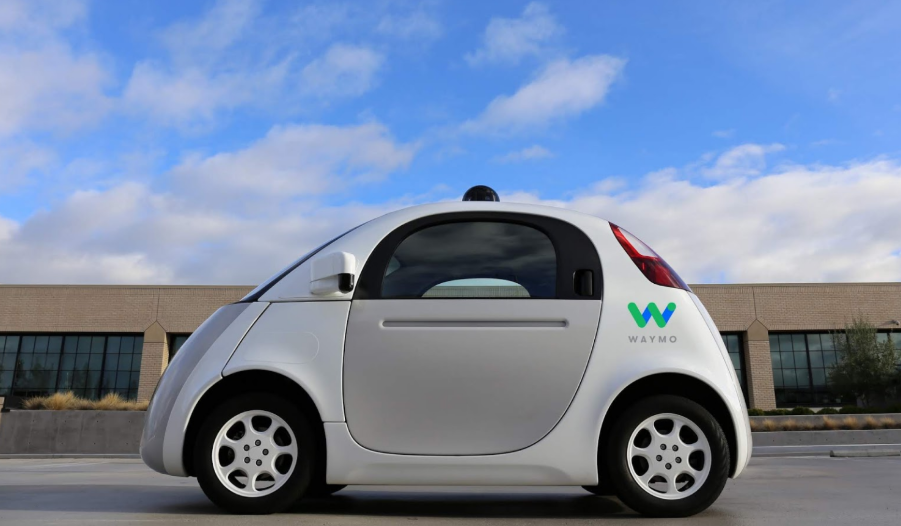
\includegraphics[width=8cm]{figs/introducción/waymo.png}
\end{center}
\caption{\textit{Waymo}, el vehículo autónomo desarrollado por \textit{Google}.}
\label{waymo}
\end{figure}

Un claro ejemplo son sus robo-taxis\footnote{\url{https://www.youtube.com/watch?v=JHgr9SgeicM}}, los cuales están ganando popularidad en ciertos estados de Estados Unidos, como San Francisco y Phoenix, donde se han desplegado flotas de estos vehículos sin conductor para transporte de pasajeros. A pesar de la alta demanda, las listas de espera para probar estos taxis autónomos y el gran interés que han generado por su potencial para revolucionar el transporte urbano, también han suscitado debates sobre su regulación, seguridad y el impacto en el empleo dentro del sector del transporte. A finales de 2024, \textit{Waymo} ya había recibido numerosos informes documentando más de 600 incidencias en las que se han visto involucrados sus robo-taxis. Por ejemplo, en febrero de 2024, uno de estos robo-taxis atropelló a un ciclista en San Francisco, y en diciembre de este mismo año dos de ellos chocaron contra un camión que estaba siendo remolcado de la carretera \cite{waymo-wiki}. 

Por otro lado, los robo-taxis \textit{Waymo} enfrentan desafíos operativos en condiciones climáticas adversas, especialmente durante lluvias intensas como las que se dan en Florida. Actualmente, se están realizando estudios y pruebas para mejorar el rendimiento de estos vehículos en tales situaciones, ya que los sensores a menudo captan demasiado ruido, y las condiciones excepcionales de las carreteras pueden llevar a otros conductores a comportarse de manera impredecible para los vehículos autónomos \cite{waymo-florida}.

\subsubsection{Autopilot de Tesla}

\textit{Tesla} ha logrado un avance significativo con su sistema \textit{Autopilot}, lanzado por primera vez en 2015, capaz de mantener un control preciso utilizando sofisticados algoritmos de \ac{IA} para tomar decisiones rápidas y precisas. Modelos como el \textit{Model 3} y el \textit{Model Y} incorporan el sistema \textit{Tesla Vision}, que prescinde del uso de radar y \ac{LiDAR}, utilizando un avanzado conjunto de cámaras junto con el procesamiento de redes neuronales desarrolladas por \textit{Tesla}. Este sistema ofrece tres niveles principales: Piloto automático, Piloto automático mejorado y Capacidad de conducción autónoma total.

El sistema de conducción autónoma de \textit{Tesla} ofrece varias funcionalidades que mejoran la experiencia de conducción en distintos niveles. El \textit{Piloto Automático} básico incluye el control de crucero adaptativo al tráfico y el autogiro, que permite mantener el vehículo dentro de un carril claramente delimitado. El \textit{Piloto Automático Mejorado} añade características como el cambio automático de carril, el cual se inicia cuando el conductor activa el intermitente, y la versión \textit{Beta} de su piloto automático, que mejora esta funcionalidad proporcionando orientación activa para transitar desde la incorporación hasta la salida de autovías, incluyendo sugerencias de cambio de carril y asistencia en intersecciones. También incorpora \textit{Autopark}, que automatiza el estacionamiento en paralelo o perpendicular, \textit{Dumb Summon}, el cual permite mover el vehículo dentro y fuera de plazas de aparcamiento estrechas mediante la aplicación móvil, y \textit{Actually Smart Summon}, que mejora las capacidades del vehículo para moverse de manera autónoma en entornos complejos, maniobrando alrededor de obstáculos y localizando al conductor dentro del área cercana. Finalmente, la \textit{Capacidad de Conducción Autónoma Total} integra todas las funcionalidades del Piloto Automático básico y del Piloto Automático Mejorado, agregando el control de semáforos en rojo y señales de \textit{stop}, ajusta automáticamente la velocidad y se detiene cuando el vehículo se acerca a ellos.

\begin{figure}[ht]
\begin{center}
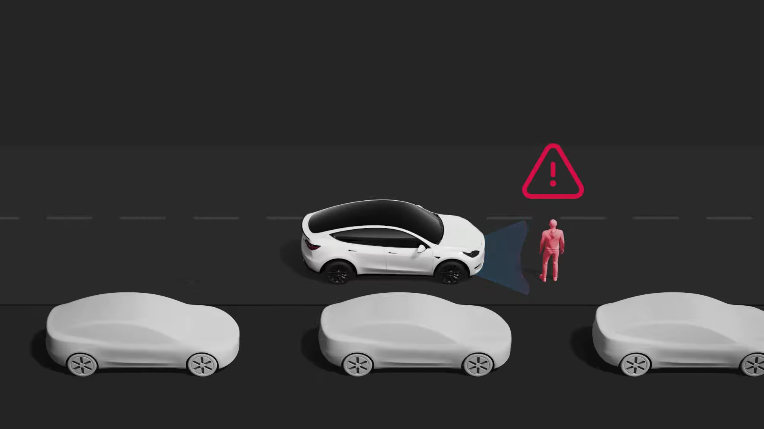
\includegraphics[width=8cm]{figs/introducción/tesla_model_y.png}
\end{center}
\caption{\textit{Tesla Model Y} frenando ante un obstáculo \cite{tesla-modely}.}
\label{tesla}
\end{figure}

A pesar de las mejoras en el rendimiento que ofrecen estas características, no hacen que el vehículo sea completamente autónomo. Aún requieren que el conductor esté completamente atento, con las manos en el volante y listo para tomar el control en cualquier momento, por lo tanto, nos encontramos en un nivel 3 de autonomía \cite{tesla-autopilot}.

El sistema \textit{Autopilot} de \textit{Tesla}, a pesar de ser altamente avanzado, presenta diversas limitaciones que pueden comprometer su rendimiento en situaciones específicas. Entre estas se incluyen curvas cerradas, cambios de elevación, señales de tráfico poco claras, condiciones de visibilidad deficiente y la interferencia causada por luz brillante o túneles. Además, la dirección automática puede fallar si las marcas de los carriles son poco visibles, están mal mantenidas o si el sistema de cámaras o sensores se encuentra obstruido, cubierto o dañado. El cambio automático de carril, por otro lado, no debe utilizarse en carreteras con tráfico constante ni en aquellas con presencia de bicicletas o peatones. \textit{Tesla} advierte en sus manuales de uso sobre estas limitaciones en cada modelo y subraya la necesidad de que el conductor se mantenga completamente atento, enfatizando que el sistema no es 100\% fiable en todas las situaciones que pueden darse durante la conducción \cite{tesla-limitations}.

Las últimas versiones de \textit{Tesla} solo incluyen el uso de cámaras para la percepción, prescindiendo del uso de tecnologías como el \ac{LiDAR} y el radar. Esto puede ser peligroso para circulación, pues las cámaras dependen en gran medida de luz y el clima, generando situaciones de riesgo en ocasiones de baja visibilidad o condiciones meteorológicas adversas. En contraste, el \ac{LiDAR} y el radar son menos susceptibles a este tipo de situaciones y pueden aportar una percepción más fiable, complementando la información de las cámaras para una detección más precisa.

\subsubsection{Cruise}

\textit{Cruise}, una empresa subsidiaria de \textit{General Motors}, en 2022 lanzó su servicio de taxis autónomos después de recibir la autorización de las autoridades reguladoras, permitiendo transportar pasajeros en San Francisco sin la necesidad de un conductor humano. Este servicio, que utiliza su innovador vehículo \textit{Cruise AV}, consolidó a \textit{Cruise} como pionera en la implementación de robo-taxis de nivel 4. 

El \textit{Cruise AV} sobresale por su diseño avanzado, con un 40\% de su hardware desarrollado específicamente para la conducción autónoma. Este modelo integra sensores de última generación, como cámaras, \ac{LiDAR} y radar que, combinados con \ac{RNN}, permiten un reconocimiento avanzado de obstáculos y el análisis de patrones temporales, identificando con precisión vehículos estacionados en doble fila. Según las pruebas, el \textit{Cruise AV} es capaz de realizar entre 200 y 800 maniobras diarias para sortear este tipo de obstáculos. Además, utiliza algoritmos de planificación de trayectorias inteligentes para ejecutar maniobras seguras, incluso en condiciones climáticas adversas como la lluvia \cite{cruise}.

\begin{figure}[ht]
\begin{center}
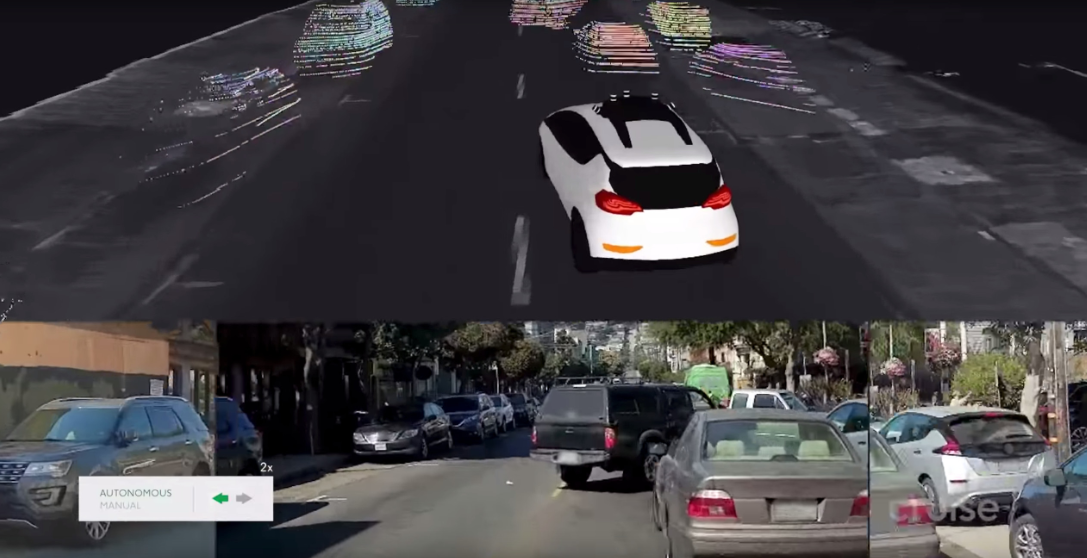
\includegraphics[width=9cm]{figs/introducción/cruise_av.png}
\end{center}
\caption{Detección de otros coches del \textit{Cruise AV} \cite{cruise-video}.}
\label{cruise}
\end{figure}

\newpage

Aunque el \textit{Cruise AV} fue diseñado para operar en entornos urbanos densos y complejos, los numerosos accidentes y problemas de tráfico ocurridos en San Francisco han puesto de manifiesto sus limitaciones. Estas incidencias llevaron a que fueran retirados de las calles de la ciudad e incluso al abandono de \textit{Cruise} en el negocio de los robo-taxis\footnote{\url{https://www.theverge.com/2024/12/10/24318259/gm-cruise-shutdown-robotaxi-super-cruise}}, evidenciando que aún queda un largo camino por recorrer para garantizar la integración segura y eficiente de los vehículos sin conductor en entornos urbanos \cite{robotaxis-cruise}.

\subsubsection{Baidu}

\textit{Baidu} es una empresa china que está revolucionando el campo de la conducción autónoma, compitiendo directamente con empresas líderes como \textit{Waymo} y \textit{Tesla}, pero ofreciendo precios significativamente más bajos. Desde 2021, la compañía ha estado desarrollando una serie de taxis autónomos y, en 2024, lanzó su sexto modelo, el \textit{Baidu RT76}. Este innovador robo-taxi está diseñado para operar sin conductor en grandes entornos urbanos, alcanzando un nivel 4 de autonomía. Destaca por sus avanzadas características tecnológicas, que incluyen cinco unidades \ac{LiDAR} y hasta cuarenta sensores de siete categorías diferentes, permitiéndole detectar y reaccionar con precisión ante su entorno. Además, utiliza \ac{IA} avanzada, respaldada por más de 100 millones de kilómetros de experiencia en conducción autónoma. Según \textit{Baidu}, su tecnología es diez veces más segura que la de un conductor humano. Actualmente, hay 500 robo-taxis \textit{Baidu RT76} circulando por las calles de Wuhan \cite{baidu}.

\begin{figure}[ht]
  \begin{center}
    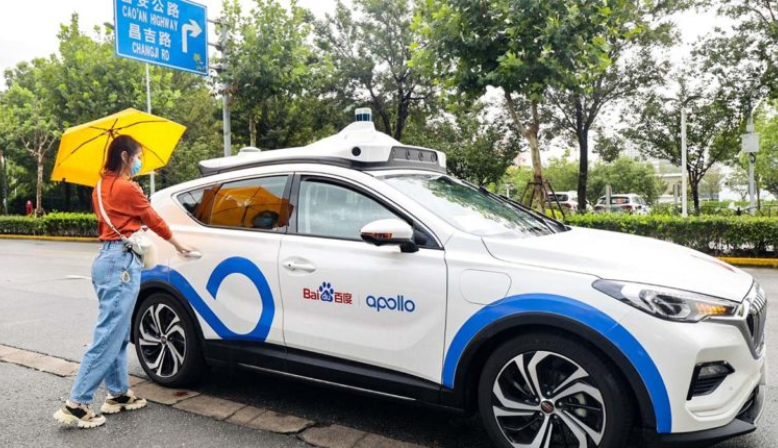
\includegraphics[width=8cm]{figs/introducción/baidu.png}
  \end{center}
  \caption{Robo-taxi autónomo \textit{Baidu RT76} \cite{foto-baidu}.}
  \label{baidu}
\end{figure}

\newpage

\subsection{Desafíos actuales en la implementación de vehículos autónomos}
\label{sec:desafíos}

Los vehículos autónomos enfrentan numerosos desafíos que deben ser superados para lograr su implementación generalizada. Estos desafíos se dividen principalmente en aspectos técnicos y no técnicos, cada uno con sus propias complejidades que requieren soluciones específicas.

En el ámbito técnico, uno de los mayores retos radica en la detección de objetos y análisis de datos. Los vehículos autónomos necesitan identificar obstáculos de manera inequívoca, incluso a altas velocidades y largas distancias. Esto exige un software avanzado capaz de procesar grandes volúmenes de datos en tiempo real con un alto grado de precisión, un área que aún enfrenta importantes limitaciones. Además, garantizar un sistema seguro y fiable implica desarrollar tecnología tolerante a fallos y capaz de operar de manera eficiente en entornos no controlados. En el mundo real, los vehículos autónomos deben enfrentarse a miles de situaciones impredecibles durante la conducción y, los sistemas actuales, todavía están lejos de resolver de manera eficiente todas estas incertidumbres. Otro desafío técnico crucial es la seguridad cibernética. Los vehículos autónomos, especialmente aquellos basados en \ac{DL}, son vulnerables a ataques que podrían comprometer su funcionalidad o la seguridad de sus ocupantes. Por ello, es imprescindible implementar estrategias robustas de defensa para mitigar estos riesgos y generar confianza en la tecnología.

En el ámbito no técnico, las cuestiones legales y éticas presentan una barrera importante. Existe una preocupación creciente sobre la responsabilidad en caso de accidentes, ya que no está claro si la culpa recaería en el fabricante, el desarrollador del software o el propietario del vehículo. También es importante salvaguardar la privacidad de los datos de los pasajeros, ya que los sistemas autónomos recopilan y procesan grandes cantidades de información personal.

La aceptación por parte de los consumidores y las regulaciones gubernamentales son factores determinantes en el desarrollo de vehículos autónomos. En la actualidad, las políticas y normativas suelen avanzar más lento que el desarrollo tecnológico, lo que complica las validaciones y la implementación a gran escala. Además, las pruebas de estos vehículos en entornos urbanos pueden afectar gravemente a la población, provocando descontento o incluso situaciones de riesgo si no se gestionan adecuadamente. Este desajuste entre innovación tecnológica y regulación es una de las razones por las cuales los vehículos autónomos aún enfrentan desafíos a nivel social.

Un ejemplo evidente de la incomodidad social ante los vehículos autónomos se da en San Francisco, California, donde las flotas de robotaxis de \textit{Waymo} (de \textit{Google}) y \textit{Cruise} (de \textit{General Motors}) han generado numerosos problemas. Inicialmente, los taxis autónomos de \textit{Waymo} fueron bien recibidos por los habitantes, pero pronto surgieron inconvenientes que transformaron la expectativa en frustración. Para estos vehículos, se habilitó un estacionamiento rodeado de viviendas, donde los robo-taxis esperan a ser contratados. Durante este proceso, sus sistemas activan la bocina al detectar la proximidad de otros vehículos, creando ruido constante que ha exasperado a los vecinos. Esta función, diseñada originalmente para prevenir accidentes, se ha convertido en uno los mayores inconvenientes de los robo-taxis de \textit{Waymo} \cite{robotaxis-waymo}. También han recibido una gran cantidad de reportes y quejas sobre problemas que han ocasionado en las carreteras. Siendo la más grave un accidente que provocó una víctima mortal el 19 de enero de 2025, cuando un robo-taxi colisionó contra un \textit{Tesla} que viaja a 158km/h \cite{waymo-wiki}.

Por su parte, los robo-taxis de \textit{Cruise} han enfrentado críticas aún más severas, culminando en su retirada indefinida de las calles de San Francisco y la renuncia de esta empresa al desarrollo de taxis sin conductor. Estos vehículos han causado repetidas obstrucciones en el tráfico, especialmente en intersecciones, lo que ha obligado a movilizar a los servicios de bomberos en numerosas ocasiones. Además, los vehículos de \textit{Cruise} se han visto implicados en varios accidentes, siendo el más grave el atropello a una mujer a finales de 2023. En este incidente, el robo-taxi arrastró a la víctima varios metros antes de detenerse, complicando su remoción y marcando el punto crítico que llevó a su retirada \cite{robotaxis-cruise}.

La superación de estos obstáculos requerirá soluciones innovadoras que satisfagan las necesidades de los consumidores, la industria y los gobiernos. La colaboración interdisciplinaria es clave para abordar estos desafíos, sentando las bases de un futuro en el que los vehículos autónomos sean seguros, eficientes y ampliamente aceptados en la sociedad \cite{challenges-autonomous}.

\section{Impacto de la IA en vehículos autónomos}
\label{sec:ia-intro}

Los coches autónomos son sistemas diseñados para tomar decisiones sin la intervención humana, procesando flujos de datos procedentes de diversas fuentes a bordo, como cámaras, radares, \ac{LiDAR}, sensores ultrasónicos, unidades \ac{GPS} y sensores inerciales. Estos sistemas utilizan las observaciones recogidas para interpretar el entorno y tomar decisiones sobre la conducción del vehículo, respondiendo de manera adecuada a las situaciones que se presenten en la carretera. A través de los actuadores, el sistema de control ejecuta estas decisiones realizando maniobras como el giro del volante, la activación de los frenos o el ajuste del acelerador.

La información procesada por los sensores puede interpretarse de diversas maneras, utilizando métodos tradicionales basados en reglas predefinidas y sistemas matemáticos, o enfoques más avanzados basados en \ac{IA}. En el pasado, los algoritmos necesarios para la visión computacional y la toma de decisiones en conducción autónoma eran altamente costosos a nivel computacional, lo que impedía su respuesta en tiempo real y representaba un desafío crucial para este campo. Además, estos métodos tradicionales se basan en reglas predefinidas y sistemas matemáticos que no son adecuados para situaciones reales, donde la incertidumbre es un factor clave. Sin embargo, los avances en la \ac{IA} han permitido mejorar significativamente este aspecto, ofreciendo soluciones más rápidas y eficientes que posibilitan la toma de decisiones en tiempo real con un alto grado de fiabilidad y precisión. Estos modelos son capaces de gestionar esta información de forma más eficiente, adaptándose a las variaciones en el entorno y mejorando el rendimiento del sistema.

Existen diversas soluciones en el ámbito de la \ac{IA} y, en la actualidad, las basadas en \ac{ML} están ganando cada vez más popularidad. Esto se debe a su capacidad para mejorar continuamente el rendimiento del sistema mediante el aprendizaje de la experiencia y su adaptación a nuevas situaciones. Existen diferentes tipos de \ac{ML} dependiendo de cómo se realicen los entrenamientos.

\begin{figure}[ht]
\begin{center}
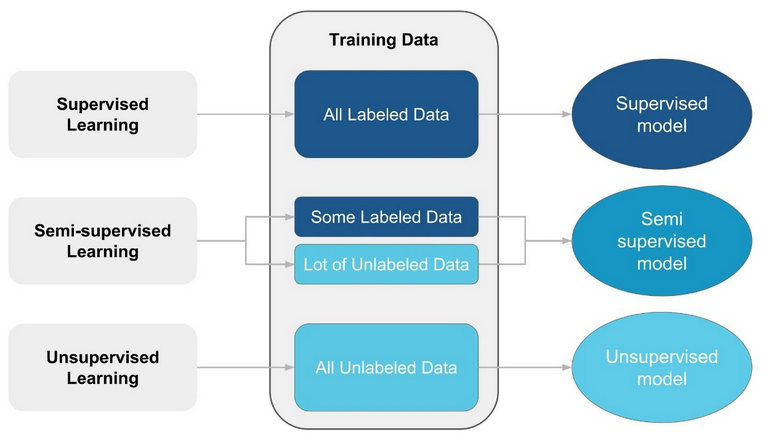
\includegraphics[width=8cm]{figs/introducción/training_type.png}
\end{center}
\caption{Tipos de \ac{ML} \cite{foto-ml}.}
\label{ml}
\end{figure}

\subsection{Aprendizaje supervisado}

El aprendizaje supervisado se basa en algoritmos diseñados para clasificar o predecir resultados utilizando un conjunto de datos etiquetados, en el que cada entrada tiene una salida asociada que representa la respuesta correcta. Durante el proceso de entrenamiento, el modelo ajusta sus parámetros al analizar estos datos, buscando minimizar el error entre sus predicciones y las respuestas correctas. Este tipo de aprendizaje requiere un análisis previo de los datos de entrenamiento para identificar las características relevantes que deben ser extraídas. El objetivo principal es predecir etiquetas para datos no vistos anteriormente, siendo ampliamente utilizado en tareas de clasificación y regresión. La precisión del modelo depende en gran medida de la calidad de los \textit{datasets} \cite{supervised-learning}.

En el ámbito de la conducción autónoma, el aprendizaje supervisado juega un papel crucial, especialmente en la detección de objetos como peatones, señales de tráfico, otros vehículos o la carretera. Un algoritmo destacado para esta tarea es \ac{YOLO}, un modelo de detección de objetos en imágenes o videos en tiempo real basado en \ac{CNN}. A diferencia de otros métodos que realizan la detección en múltiples etapas, \ac{YOLO} integra la localización, segmentación y clasificación en un solo modelo, haciéndolo extremadamente rápido y eficiente. \ac{YOLO} utiliza lo que se conoce como \textit{bounding boxes} para marcar los límites de los objetos detectados en la imagen o video \cite{yolo}. Otros modelos, como \textit{EfficientVit}, amplían la clasificación de imágenes, pasando de predicciones a nivel de imagen a predicciones a nivel de píxel, lo que resulta muy útil para identificar con exactitud, por ejemplo, los límites de la calzada. \textit{Tesla} también utiliza \ac{CNN} en su sistema \textit{Autopilot} para tareas de percepción visual\footnote{\url{https://www.tesla.com/es_es/AI}}. Todos los coches de \textit{Tesla} colaboran para crear una gran base de datos que sirve para entrenar sus redes neuronales \cite{tesla-dataset}. 

\begin{figure}[ht]
\begin{center}
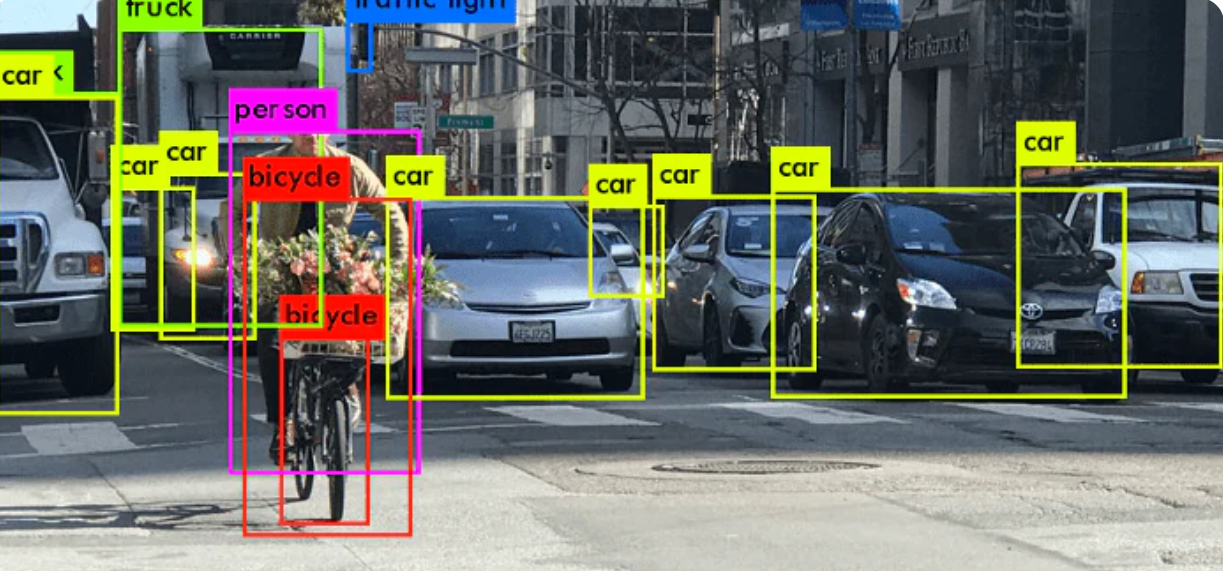
\includegraphics[width=8cm]{figs/introducción/yolo.png}
\end{center}
\caption{YOLO identificación de objetos en la carretera \cite{yolo-detection}.}
\label{yolo}
\end{figure}

Existen otro tipo de modelos basados en \textit{imitation learning}, en el los que el agente aprende a realizar una tarea observando cómo la realiza un experto en ella, comúnmente un humano u otro modelo ya formado para ello \cite{imitation-learning}. El modelo \textit{ChauffeurNet} de \textit{Waymo} es un coche autónomo basado en \textit{imitation learning} que toma como entrada imágenes segmentadas semánticamente. Este modelo se entrena con demostraciones humanas y otros escenarios de conducción difíciles generados artificialmente, esta combinación logra que \textit{ChauffeurNet} ofrezca una conducción autónoma segura y eficiente hasta en situaciones inesperadas \cite{chauffeurnet-paper}.

\subsection{Aprendizaje semi-supervisado}

El aprendizaje semi-supervisado combina datos etiquetados y no etiquetados en el conjunto de entrenamiento. Este enfoque resulta especialmente útil cuando el etiquetado de datos es costoso o difícil de realizar en grandes cantidades. A diferencia del aprendizaje supervisado tradicional, permite obtener buenos resultados utilizando solo un pequeño conjunto de ejemplos etiquetados, haciéndolo más eficiente y práctico en determinados escenarios. Además, este enfoque refleja de manera más cercana cómo las personas aprenden a partir de una combinación de ejemplos explícitos y observaciones generales \cite{semi}.

Existe una innovadora tecnología basada en algoritmos de aprendizaje semi-supervisado, cuyo objetivo es la fusión de datos entre nubes de puntos del \ac{LiDAR} e imágenes para mejorar la detección de objetos en 3D en vehículos autónomos. El etiquetado manual de datos \ac{LiDAR} e imágenes es costoso y requiere mucho tiempo, lo que hace que este enfoque sea más accesible. Esta nueva perspectiva mejora la capacidad del modelo para generalizar y adaptarse a nuevos entornos o condiciones no vistas durante el entrenamiento, lo cual es crucial en la conducción autónoma, donde los vehículos deben operar de manera robusta en situaciones cambiantes. Los resultados muestran que el uso de aprendizaje semi-supervisado no solo optimiza los costos y tiempos de entrenamiento, sino que también incrementa la precisión de la detección en 3D, haciendo que la tecnología sea más escalable y eficiente \cite{semi-ex}.

\subsection{Aprendizaje no supervisado}

El aprendizaje no supervisado opera en conjuntos de datos sin etiquetas, donde el propio modelo es capaz de identificar patrones y estructuras, agrupando los datos en categorías o clústeres. Las tareas principales incluyen el \textit{clustering}, la reducción de dimensionalidad y la asociación, que busca identificar relaciones o reglas frecuentes entre variables dentro de un conjunto de datos. Este método puede ser más rentable que el aprendizaje supervisado, ya que no requiere la creación y etiquetado de grandes conjuntos de datos de entrenamiento. En este tipo de aprendizaje, la calidad de los resultados depende en gran medida de la elección adecuada del algoritmo y los parámetros de entrenamiento utilizados \cite{no-supervised-learning}.

\subsubsection{Aprendizaje por refuerzo}
\label{sec:refuerzo}

El aprendizaje por refuerzo es un enfoque de aprendizaje no supervisado donde un agente toma decisiones dentro de un entorno definido, buscando maximizar la recompensa final que recibe a lo largo del tiempo. Durante los entrenamientos, el agente observa su estado actual en el entorno, elige una acción basada en una política y recibe una recompensa. Utilizando esta retroalimentación, el agente ajusta su política para predecir las mejores acciones en cada estado, teniendo en cuenta tanto las recompensas inmediatas como las futuras. De esta forma, construye una tabla que mapea los estados con las acciones llamada \textit{Q-table}, apuntando la recompensa que proporciona cada acción dado un estado concreto. Este proceso logra un equilibrio entre la exploración, probar nuevas acciones para obtener más información sobre el entorno, y la explotación, elegir las mejores acciones basadas en la experiencia previa.

\begin{figure}[ht]
\begin{center}
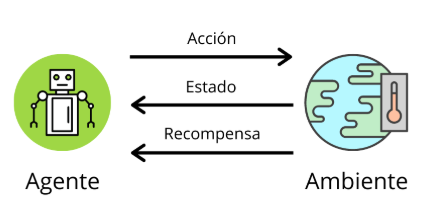
\includegraphics[width=7cm]{figs/introducción/RL.png}
\end{center}
\caption{Esquema del proceso de aprendizaje por refuerzo \cite{reinforcement-learning-schema}.}
\label{rl}
\end{figure}

En el contexto de la conducción autónoma, el aprendizaje por refuerzo se aplica de manera efectiva en sistemas como \textit{AWS DeepRacer}, donde un coche autónomo se entrena para navegar por una pista de carreras\footnote{\url{https://burjcdigital.urjc.es/items/2951749e-f6a8-4369-a543-8be924a8fee9}\\ \url{https://burjcdigital.urjc.es/items/f6ce4e69-199b-4f73-a136-0f4782eac351}}. A través de la simulación, el vehículo explora diversas acciones, como ajustar su velocidad o realizar giros, con el objetivo de maximizar su rendimiento en el circuito. Al principio, el agente toma decisiones aleatorias, pero a medida que recibe retroalimentación en forma de recompensas, como avanzar por la carretera sin salirse o completar la carrera en el menor tiempo posible, ajusta su política de conducción para tomar decisiones más acertadas y optimizar su desempeño. Este proceso de aprendizaje es continuo, permitiendo al coche mejorar su capacidad para manejar diversas condiciones de la pista, combinando la exploración de nuevas tácticas con la explotación de las que ya han demostrado ser eficaces \cite{aws-deep-racer}.

\begin{figure}[ht]
\begin{center}
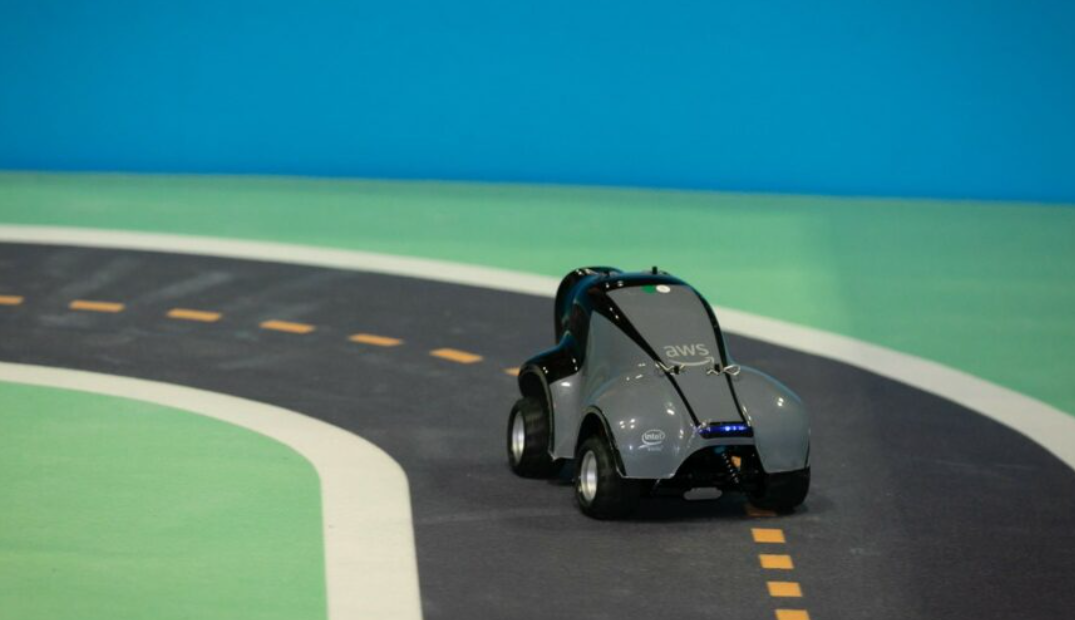
\includegraphics[width=7cm]{figs/introducción/aws_racer.png}
\end{center}
\caption{Modelo \textit{AWS DeepRacer} \cite{aws-deepracer}.}
\label{aws}
\end{figure}

Cada uno de estos enfoques de \ac{ML} tiene sus propias fortalezas y limitaciones. Sin embargo, en la mayoría de los sistemas autónomos modernos, se combinan varias técnicas para garantizar que el vehículo pueda adaptarse a una amplia variedad de condiciones de tráfico y entornos. Al integrar estas soluciones, los coches autónomos pueden mejorar continuamente su rendimiento y fiabilidad.

Para crear nuestro sistema de conducción autónoma nos centraremos en el \ac{DRL}, ya que, como se comprobó en anteriores \ac{TFG} basados en aprendizaje por refuerzo\footnote{\url{https://burjcdigital.urjc.es/items/f6ce4e69-199b-4f73-a136-0f4782eac351}}, donde el agente guarda la relación entre estados y acciones en una tabla, no escalaban bien para escenarios complejos como el de conducción autónoma. No es práctico almacenar en una tabla las relaciones entre estados y observaciones, ya que sería necesario explorar cada estado al menos una vez para encontrar la solución más óptima. Por ello, se ha empezado directamente con algoritmos basados en \ac{DRL}. En su lugar, estos algoritmos usan redes neuronales diseñadas para aprender la función que mapea estados-acciones. Estas redes son capaces de estimar el valor de estados no explorados, ya que aprenden las relaciones entre los diferentes pares estado-acción. Esto permite a los algoritmos basados en \ac{DRL} generalizar de manera más eficiente, mejorar su rendimiento en entornos complejos donde las reglas no son evidentes y adaptarse a nuevas situaciones sin necesidad de explorar cada uno de los estados de forma explícita. Por ejemplo, aunque hayan sido entrenadas con curvas de 30º o menos, los modelos resultantes son capaces de generalizar y tomar adecuadamente una curva de 40º.

Este \ac{TFG} propone una solución que combina el aprendizaje supervisado para la percepción, con \ac{DRL} para la toma de decisiones. El objetivo es resolver problemas como el seguimiento fluido del carril mediante diferentes técnicas de detección, mantener un control de crucero adaptativo al tráfico basado en el \ac{LiDAR} y realizar maniobras de adelantamiento, combinando la detección de carril, el \ac{LiDAR} y una red neuronal de segmentación semántica para la detección de la calzada. 


